%
\documentclass[parskip,headsepline, headtopline, %
footsepline, oneside, 12pt, headings=small]{scrreprt}
\usepackage[ngerman]{babel}
\usepackage[utf8]{inputenc}
\usepackage{color}
\usepackage{pdfpages} % To include other PDFs
\usepackage{changepage} 
% To insert dummy text
\usepackage{blindtext}
\setcounter{secnumdepth}{2}
 
% Provide a command to include pretty quotes
\usepackage{ragged2e} %justify dictum
\renewcommand*{\dictumwidth}{.5\textwidth}
\newcommand{\setChapterQuote}[3]{\setchapterpreamble[o]{%
\dictum[#2 \emph{#3}]{\justifying {#1}}}}
 
%Set font to times
\usepackage{txfonts}
 
% Define own Chapter style
% Pretty chapter pages
%------------------------------------------
\definecolor{nicered}{rgb}{.647,.129,.149}
\usepackage{soul}
\makeatletter
\newsavebox{\feline@chapter}
\newcommand\feline@chapter@marker[1][4cm]{%
\sbox\feline@chapter{%
\resizebox{!}{#1}{\fboxsep=1pt%
\colorbox{grey}{\color{white}\bfseries\sffamily\thechapter}%
}}%
\rotatebox{90}{%
\resizebox{%
\heightof{\usebox{\feline@chapter}}+\depthof{\usebox{\feline@chapter}}}%
{!}{\scshape\so\@chapapp}}\quad%
\raisebox{\depthof{\usebox{\feline@chapter}}}{\usebox{\feline@chapter}}%
}
\newcommand\feline@chm[1][4cm]{%
\sbox\feline@chapter{\feline@chapter@marker[#1]}%
\makebox[0pt][l]{% aka \rlap
\makebox[1cm][r]{\usebox\feline@chapter}%
}}   
 
\renewcommand*{\chapterformat}{%
\hspace{\leftmargin} \feline@chm[2.5cm] % Height of the colored box
\hspace{2cm}
}
\makeatother
%------------------------------------------
% ------------------------------------------------------------------------------
\newcommand{\HRule}[1]{\hfill \rule{0.2\linewidth}{#1}}         % Horizontal rule

\definecolor{grey}{rgb}{0.9,0.9,0.9} 

\makeatletter                                                   % Title
\def\printtitle{%                                               
    {\centering \@title\par}}
\makeatother                                                                    

\makeatletter                                                   % Author
\def\printauthor{%                                      
    {\centering \large \@author}}                               
\makeatother                                                    

% ------------------------------------------------------------------------------
% Metadata (Change this)
% ------------------------------------------------------------------------------
\title{ \fontsize{50}{60}\selectfont \\[2.10cm]
\hfill \begin{huge}{\fontfamily{@arialn}\selectfont {\fontfamily{txtt}\selectfont The Design for all}}\end{huge}
 \hfill \large{\begin{flushright}Psychologie, Design, Emotionen\end{flushright}} \\[1.9cm]
 \hfill \small{On computable processes with an application to the Kunstproblem \textbackslash\textbackslash  Winter term 2012/2013} 
}
\author{
                \hfill Martha Rohte und Maria Meister\\  
                \hfill University of Bremen\\   
                \hfill Department of Mathematics \& Computer Science \\
        \hfill \texttt{\fontfamily{cmr}\selectfont mata@informatik.uni-bremen.de} \\
        \hfill \texttt{\fontfamily{cmr}\selectfont mmeister@informatik.uni-bremen.de} \\
}


\renewcommand{\sfdefault}{@sshlined}
\begin{document}

% ------------------------------------------------------------------------------
% Maketitle
% ------------------------------------------------------------------------------
\thispagestyle{empty}                           % Remove page numbering on this page



\colorbox{grey}{
        \parbox[t]{1.14\linewidth}{
                \printtitle 
                \vspace*{0.2cm}               
        }
}
        \vfill
\printauthor                                                            % Print the author data as defined above
\HRule{1pt}

\clearpage

\begin{abstract}

\end{abstract}
% NOTE: '?' is placeholder for selected text 
% or caret location (when no selection).


\tableofcontents
 
% Chapter A
\setChapterQuote{A thought is an idea in transit.}{Pythagoras}{582 B.C. - 497 B.C.}
\chapter{Alltagsdesign}
\section{Norman}

Der das Buch geschrieben hat, ursprünglich Psychologe, setzt er sich immer mehr mit der Benutzbarkeit zuerst von Alltagsgegenständen und auch von informatischen Produkten auseinander. Sein Buch \glqq Psychology of Everyday Things \grqq ist zu großer Beliebtheit in den Kreisen der Usability Forschung und des Designs gelangt. 

\section{Technologieparadoxon}

“Whenever the number of functions and required operations exceeds the number of controls, the design becomes arbitrary, unnatural, and complicated. 
	The same technology that simplifies life by providing more functions in each device also complicates life by making the device harder to learn, harder to use. This is the paradox of technology.”

\section{Designaspekte}
	Sichtbarkeit
	Feedback
	Mapping
	Affordanz
	Constraints
\section{Konzeptuelle Modelle}
\section{Aktion}

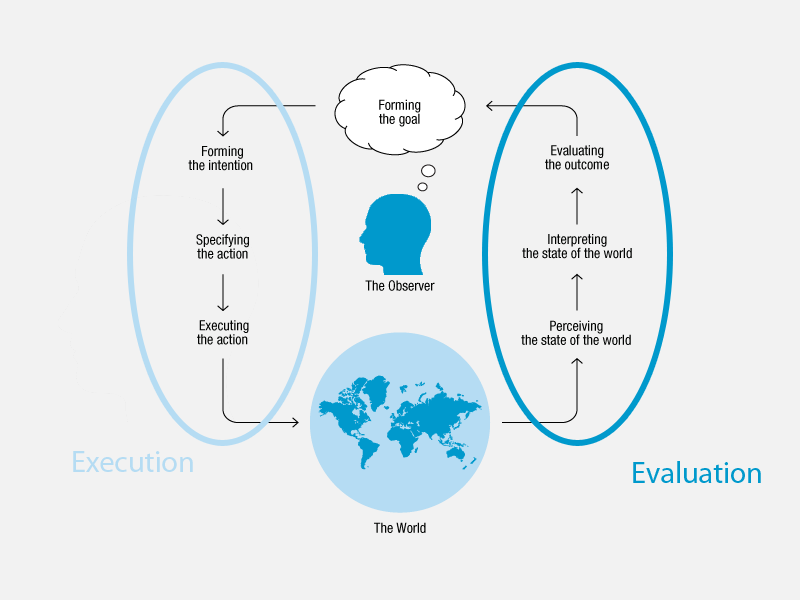
\includegraphics[width=\textwidth]{images/ActionCycle.png}

\section{Fehler}
\section{Wissen}

 
% Chapter B
\setChapterQuote{Much wisdom often goes with fewest words.}{Sophocles}{496 B.C. - 406 B.C.}
\chapter{Design und Emotion}
\section{Kansei engineering}

 
% Chapter C
\chapter{Resümee - Folgen für das Softwaredesign}
\section{Bezug auf den Kurs}
\section{Resumee}

\begin{thebibliography}{9}
	\bibitem {don} Norman, Donald (1988). The Design of Everyday Things. New York: Basic Books. ISBN 978-0-465-06710-7 
\end{thebibliography}

\end{document}
